\documentclass[../Main.tex]{subfiles}
\begin{document}
\chapter{Distributed Systems}

\intro{

}

\section{Comparison}

Goals:
\begin{enumerate}
    \item Scaling (one system is not enough)
    \item Location (move systems closer to the consumer)
    \item Fault-Tolerance (Hw will fail eventually)
\end{enumerate}

\defn{Scaling}{
    \begin{description}
        \item[Vertical] Scale systems by adding more resources to already
        existing servers. Is generally cheaper until you max out the hardware.
        No adaption of software required and is thus less complex. THe need of redundancy can pose a problem.
        \item[Horizontal] Add more nodes. In long term massive scaling
        it could be economically more feasable. It adds complexity and needs software adaption.
        The addition of fault tolerance is easier.
    \end{description}
}

\begin{figure}[H]
    \centering
    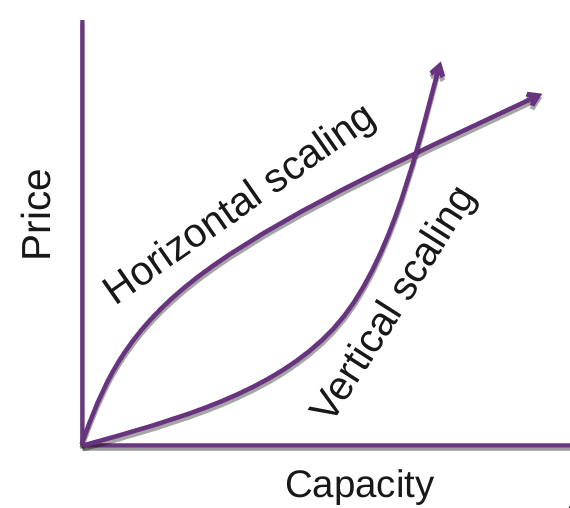
\includegraphics[width=0.25\linewidth]{Images/eco-scaling.png}
    \caption{}
\end{figure}

\defn{Some well known "laws"}{
    Moore's Law:
    \begin{itemize}
        \item The numbers of transistors doubles every 2 years.
    \end{itemize}
    Nielsen's Law:
    \begin{itemize}
        \item A high-end user's connection speed grows by 50\% per year.
    \end{itemize}
    Kryder's Law:
    \begin{itemize}
        \item Disk density douples every 13 months.
    \end{itemize}
    (Kryder's law is not applicable anymore since 2005, because consumer behaviour changed in favor of SSD's)
}

Bandwidth grows slower than compute power. Hence currently it makes sense
to prioritize the optimization of network communication.


\begin{figure}[H]
    \centering
    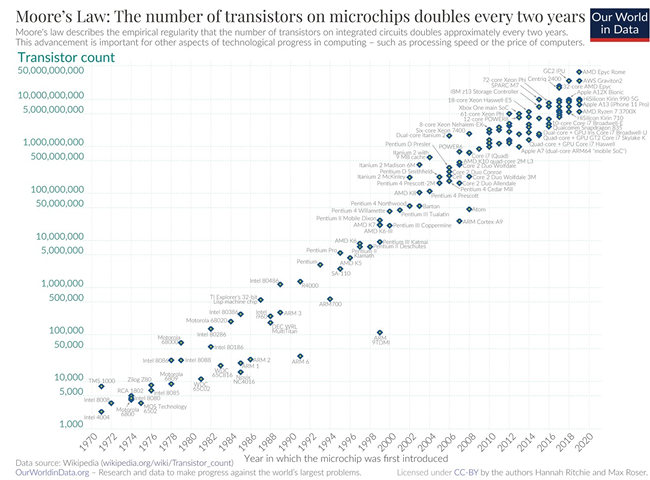
\includegraphics[width=0.5\linewidth]{Images/moore-law.png}
    \caption{Moore's Law}
\end{figure}

\begin{figure}[H]
    \centering
    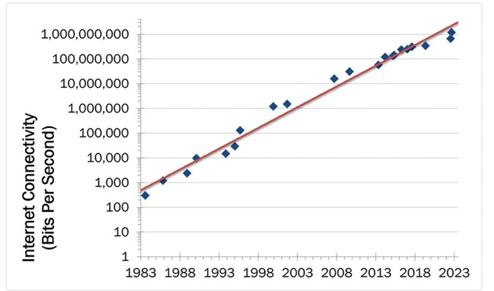
\includegraphics[width=0.5\linewidth]{Images/nielsen-law.png}
    \caption{Nielsen's Law}
\end{figure}

\end{document}
